%%==================================================================%%
%% Author : Tejedo Gonz�lez, Daniel                                 %%
%%          S�nchez Barreiro, Pablo                                 %%
%% Version: 1.0, 27/11/2012                                         %%                   %%                                                                  %%
%% Memoria del Proyecto Fin de Carrera                              %%
%% Gram�tica, pruebas                                       %%
%%==================================================================%%

\begin{figure}[t]
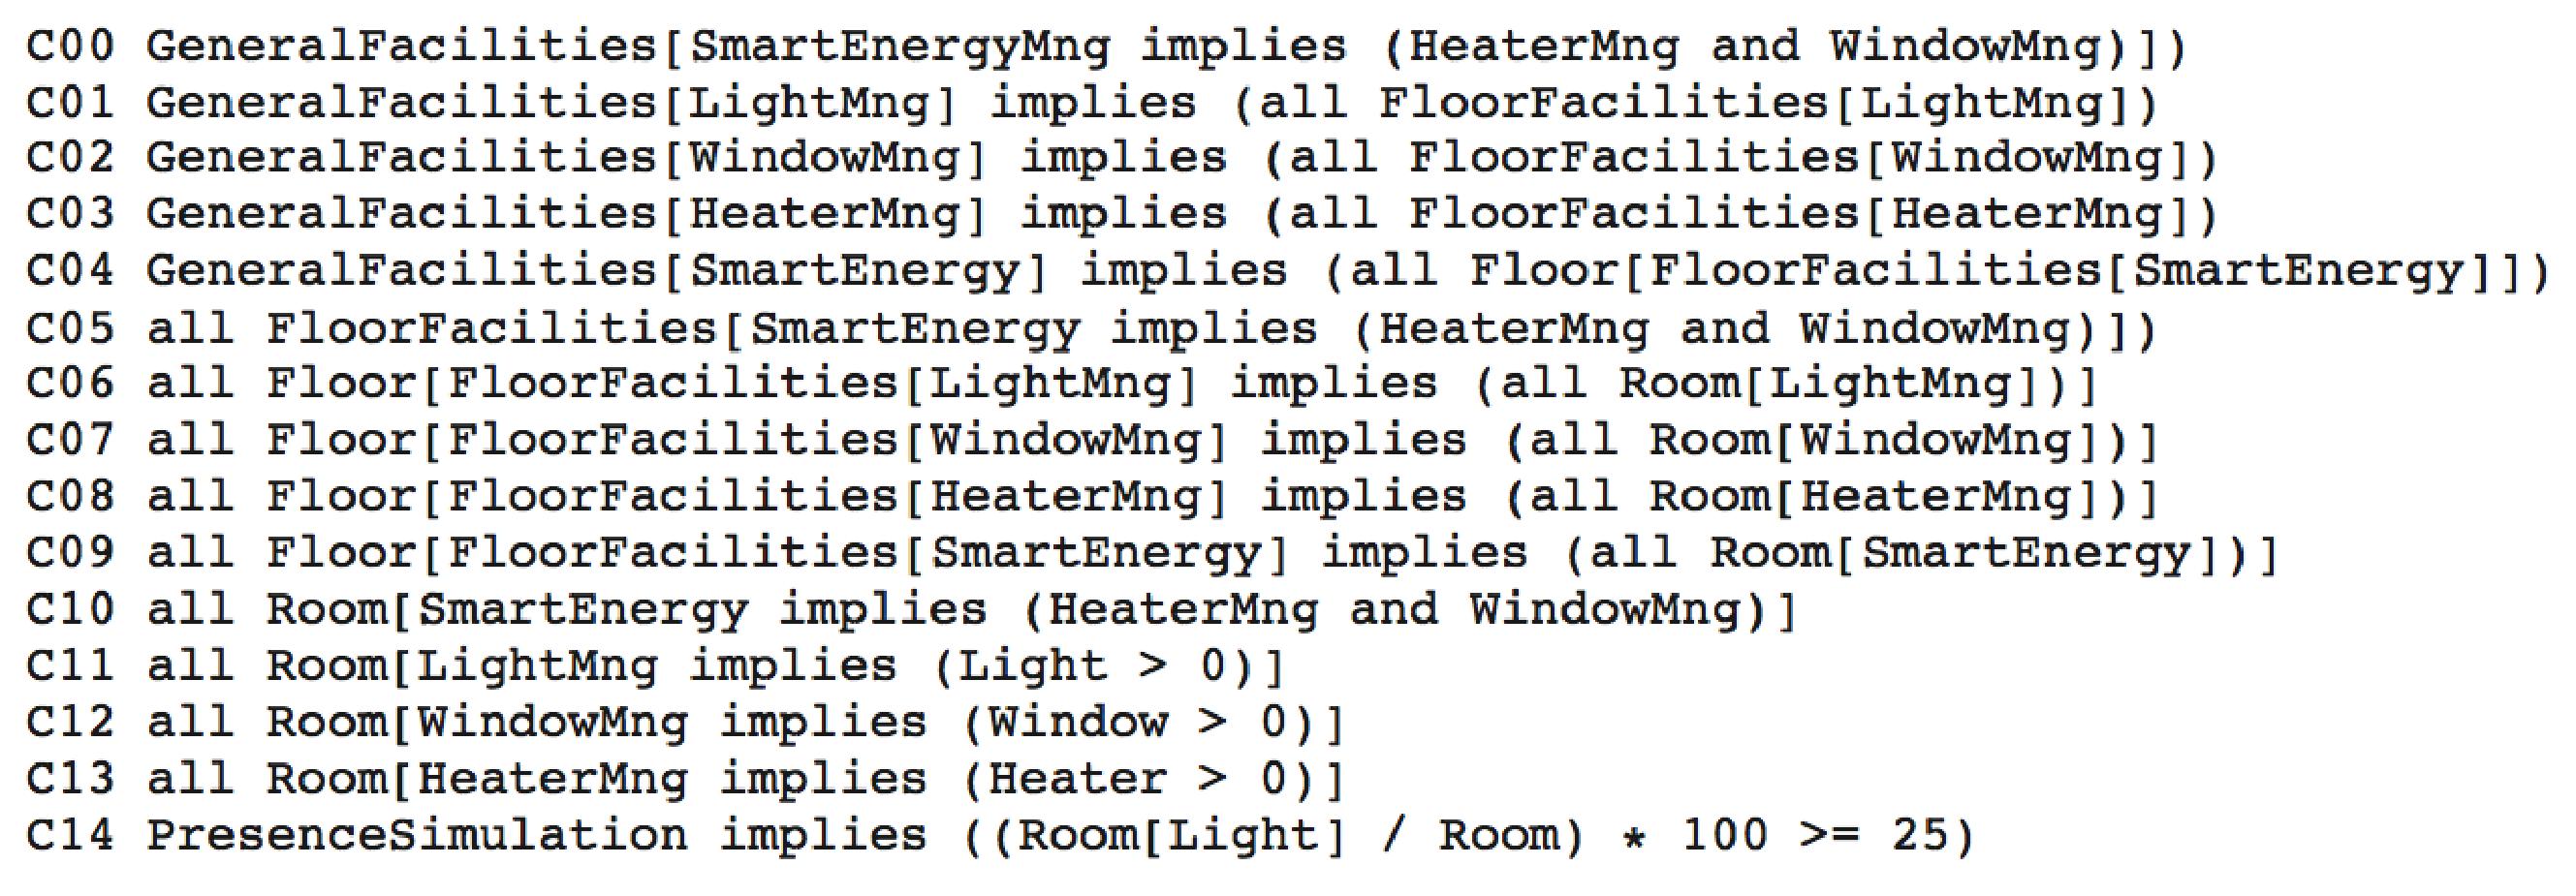
\includegraphics[scale=0.5]{gramatica/oppruebas.eps}
\caption{Bater�a de instrucciones para probar el funcionamiento de la gram�tica}
\label{figgrampruebas}
\end{figure}

Para hacer las pruebas correspondientes a la gram�tica fue de mucha utilidad la vista Outline de Eclipse, que permite obsevar el �rbol de parsing de todos los ficheros de c�digo que creemos en nuestro lenguaje. 

La bater�a de pruebas simplemente consisti� en comprobar una serie de instrucciones y observar dentro de la vista Outline si se parseaban de modo correcto. En este caso se utilizaron unas restricciones definidas en un documento previo de Hydra que conten�an todos los aspectos problem�ticos de la gram�tica, es decir, operaciones largas con prioridad y multitud de contextos. Estas instrucciones son las que se muestran en la figura \ref{figgrampruebas}. 

El resto de operaciones fueron puestas a prueba con restricciones m�s sencillitas y, como en el caso anterior, fueron exitosas. Tambi�n se usaron las instrucciones de las pruebas del cap�tulo anterior, que se pueden observar en la figura \ref{figmetains} para comprobar que el �rbol era el mismo que se cre� en ese momento.